% !TeX root = ../../thesis.tex

\section{AC Environment}
\label{sec:ac-environment}

In an AC environment, the power supply does not deliver a constant voltage.
It is a sine wave which goes from a positive voltage to a negative voltage and back again.
In the Netherlands, the RMS voltage is 230 V with a frequency of 50 Hz.
In each subsection first existing hardware will be discussed and its flaws for our purpose will be highlighted.
Then new hardware is proposed to remedy these flaws.
Finally a testbed will be showcased.





\subsection{Modulator}	

For commercial LED lighting there are fixtures available which require a DC power supply.
These fixtures often come bundled with the correct power supply, which in most cases is a SMPS (Switching Mode Power Supply).
In Figures \ref{fig:smps-current-primary-no-load} and \ref{fig:smps-current-primary-with-load} the current signature of a SMPS can be seen, without and with a load attached, respectively.
From these figures, it is clear to see that without a load, the current is not zero and with a load the current is not a constant.
This makes determining whether an LED was on or off difficult, especially if multiple of these current signatures will be superimposed.
\todo{Prob. do better conclusion why this wont work (well).}


\begin{figure}
	\centering     %%% not \center
	\subfigure[Without a load attached.]{
		\label{fig:smps-current-primary-no-load}
		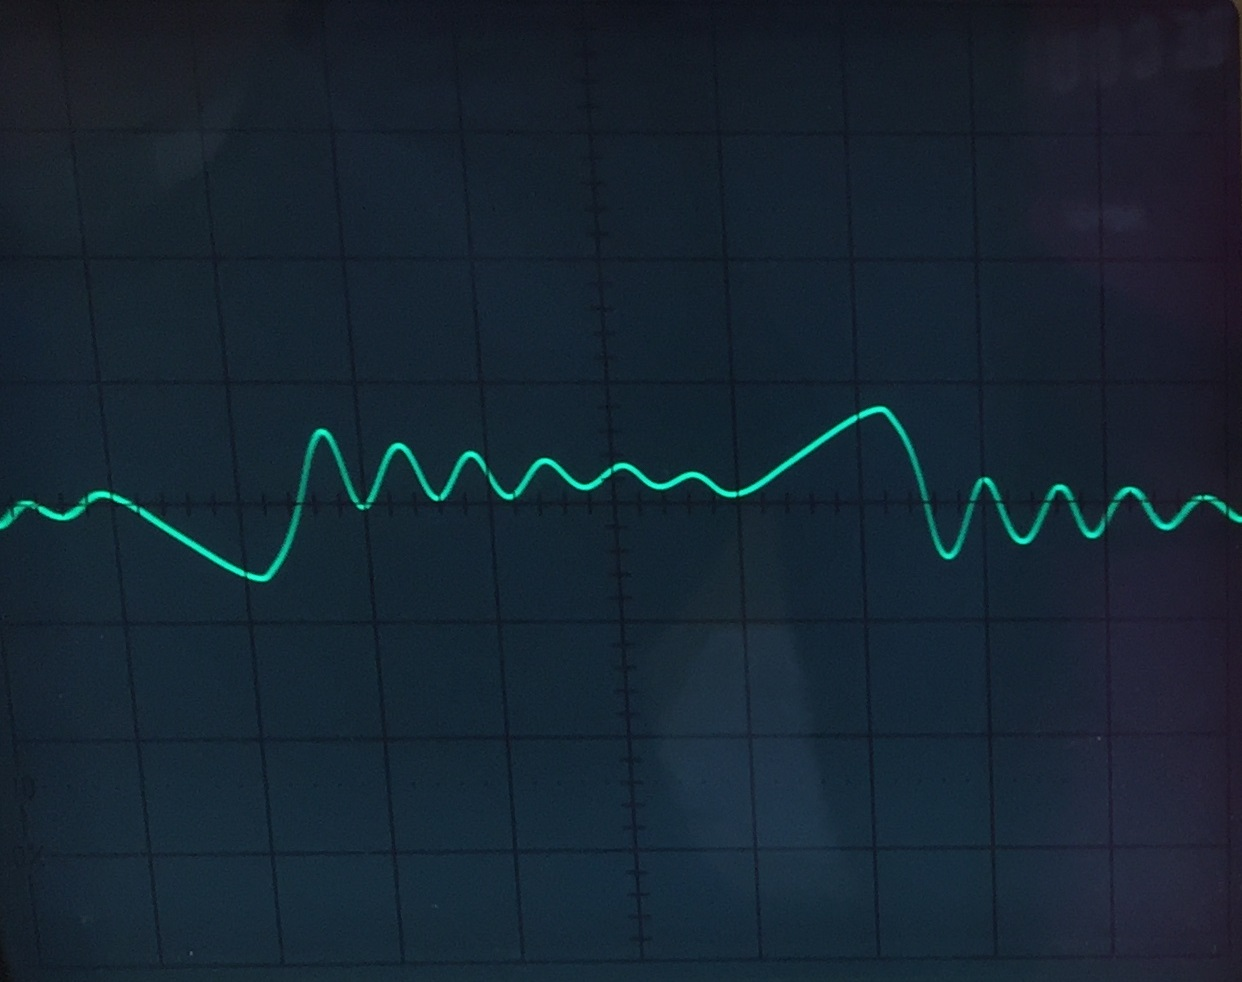
\includegraphics[width=60mm]
		{chapters/hardware-chapters/smps-current-primary-no-load-cropped.jpg}
	}
	\subfigure[With a 33 ohm resistor load attached.]{
		\label{fig:smps-current-primary-with-load}
		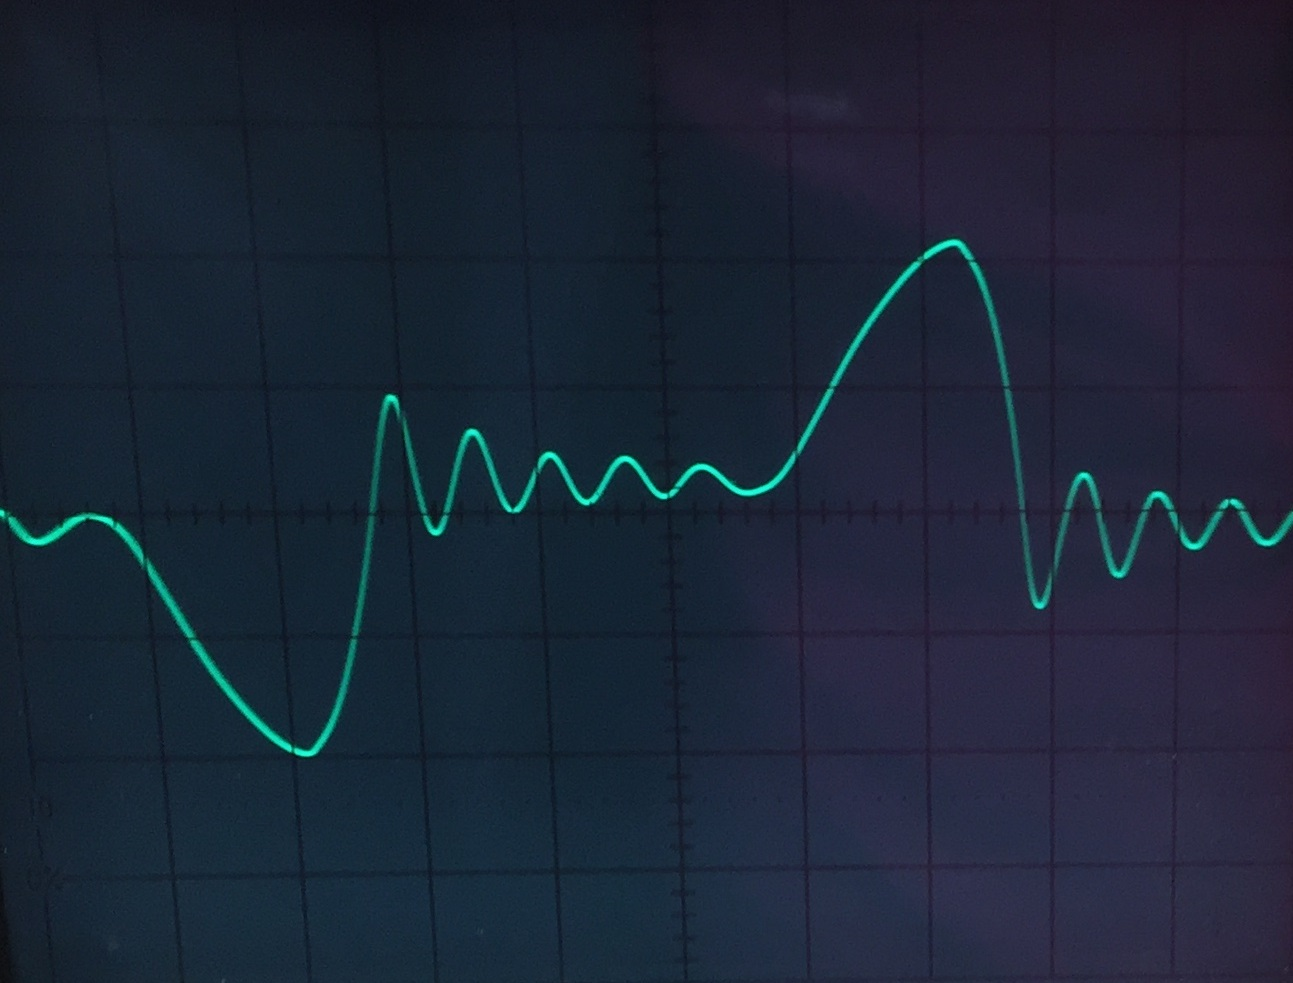
\includegraphics[width=60mm]
		{chapters/hardware-chapters/smps-current-primary-with-load-cropped.jpg}
	}

	\caption{Voltage measured over a 10 ohm series resistor at the primary side, to determine the current flow in two situations of a SMPS, with and without a load attached. Settings: 2 ms/div, 500 mV/div.}
\end{figure}



Other commercial LED lighting fixtures can be screwed directly into existing sockets and work directly via the supplied 230 V AC.
In Figures \ref{fig:commercial-230v-ac-led-on} and \ref{fig:commercial-230v-ac-led-modulating} the current signatures of this commercial 230 V AC LED can be seen, plain on and when modulated, respectively.
In order to modulate this LED, changes had to be made to the hardware that drives the actual LEDs.
In \autoref{app:commercial-230v-ac-modified-schematic} a schematic can be found, which shows the original circuit and what was modified in order to modulate the LED.









The time that is available to modulate the LED, can be seen in Figure \ref{fig:commercial-230v-ac-led-on}.
There are two peaks, each peak is 4 ms wide, for a total modulation time of 8 ms.
The AC has a period of 20 ms, so $\frac{8}{20} = 40$ \% of the time is available for modulation.
The reason for these peaks, is because at that point in time enough voltage is provided by the AC to make all those LEDs in series draw current.
In Figure \ref{fig:commercial-230v-ac-led-modulating} it can be seen that when the LED is turned off, there is no current draw.
When the LED is being turned on again, the current draw is not immediate, but takes time.
This behavior is not desired, especially not when multiple of these current signatures will be superimposed.

\begin{figure}
	\centering     %%% not \center
	\subfigure[LED is on. Settings: 5 ms/div, 1 V/div.]{
		\label{fig:commercial-230v-ac-led-on}
		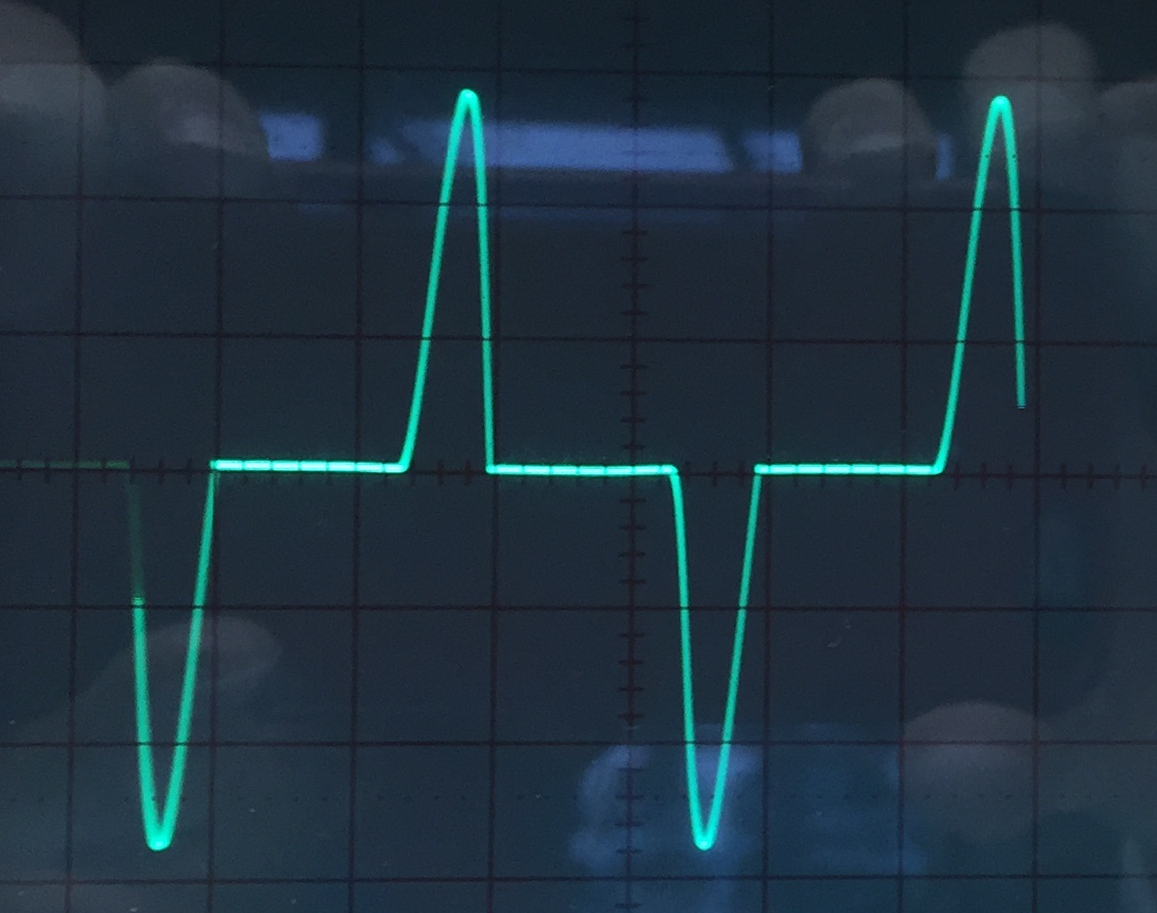
\includegraphics[width=60mm]
		{chapters/hardware-chapters/commercial-230v-ac-led-on-cropped.png}
	}
	\subfigure[LED is being modulated at 4 kHz with the other signal present in the figure. Settings: 1 ms/div, 5 V/div.]{
		\label{fig:commercial-230v-ac-led-modulating}
		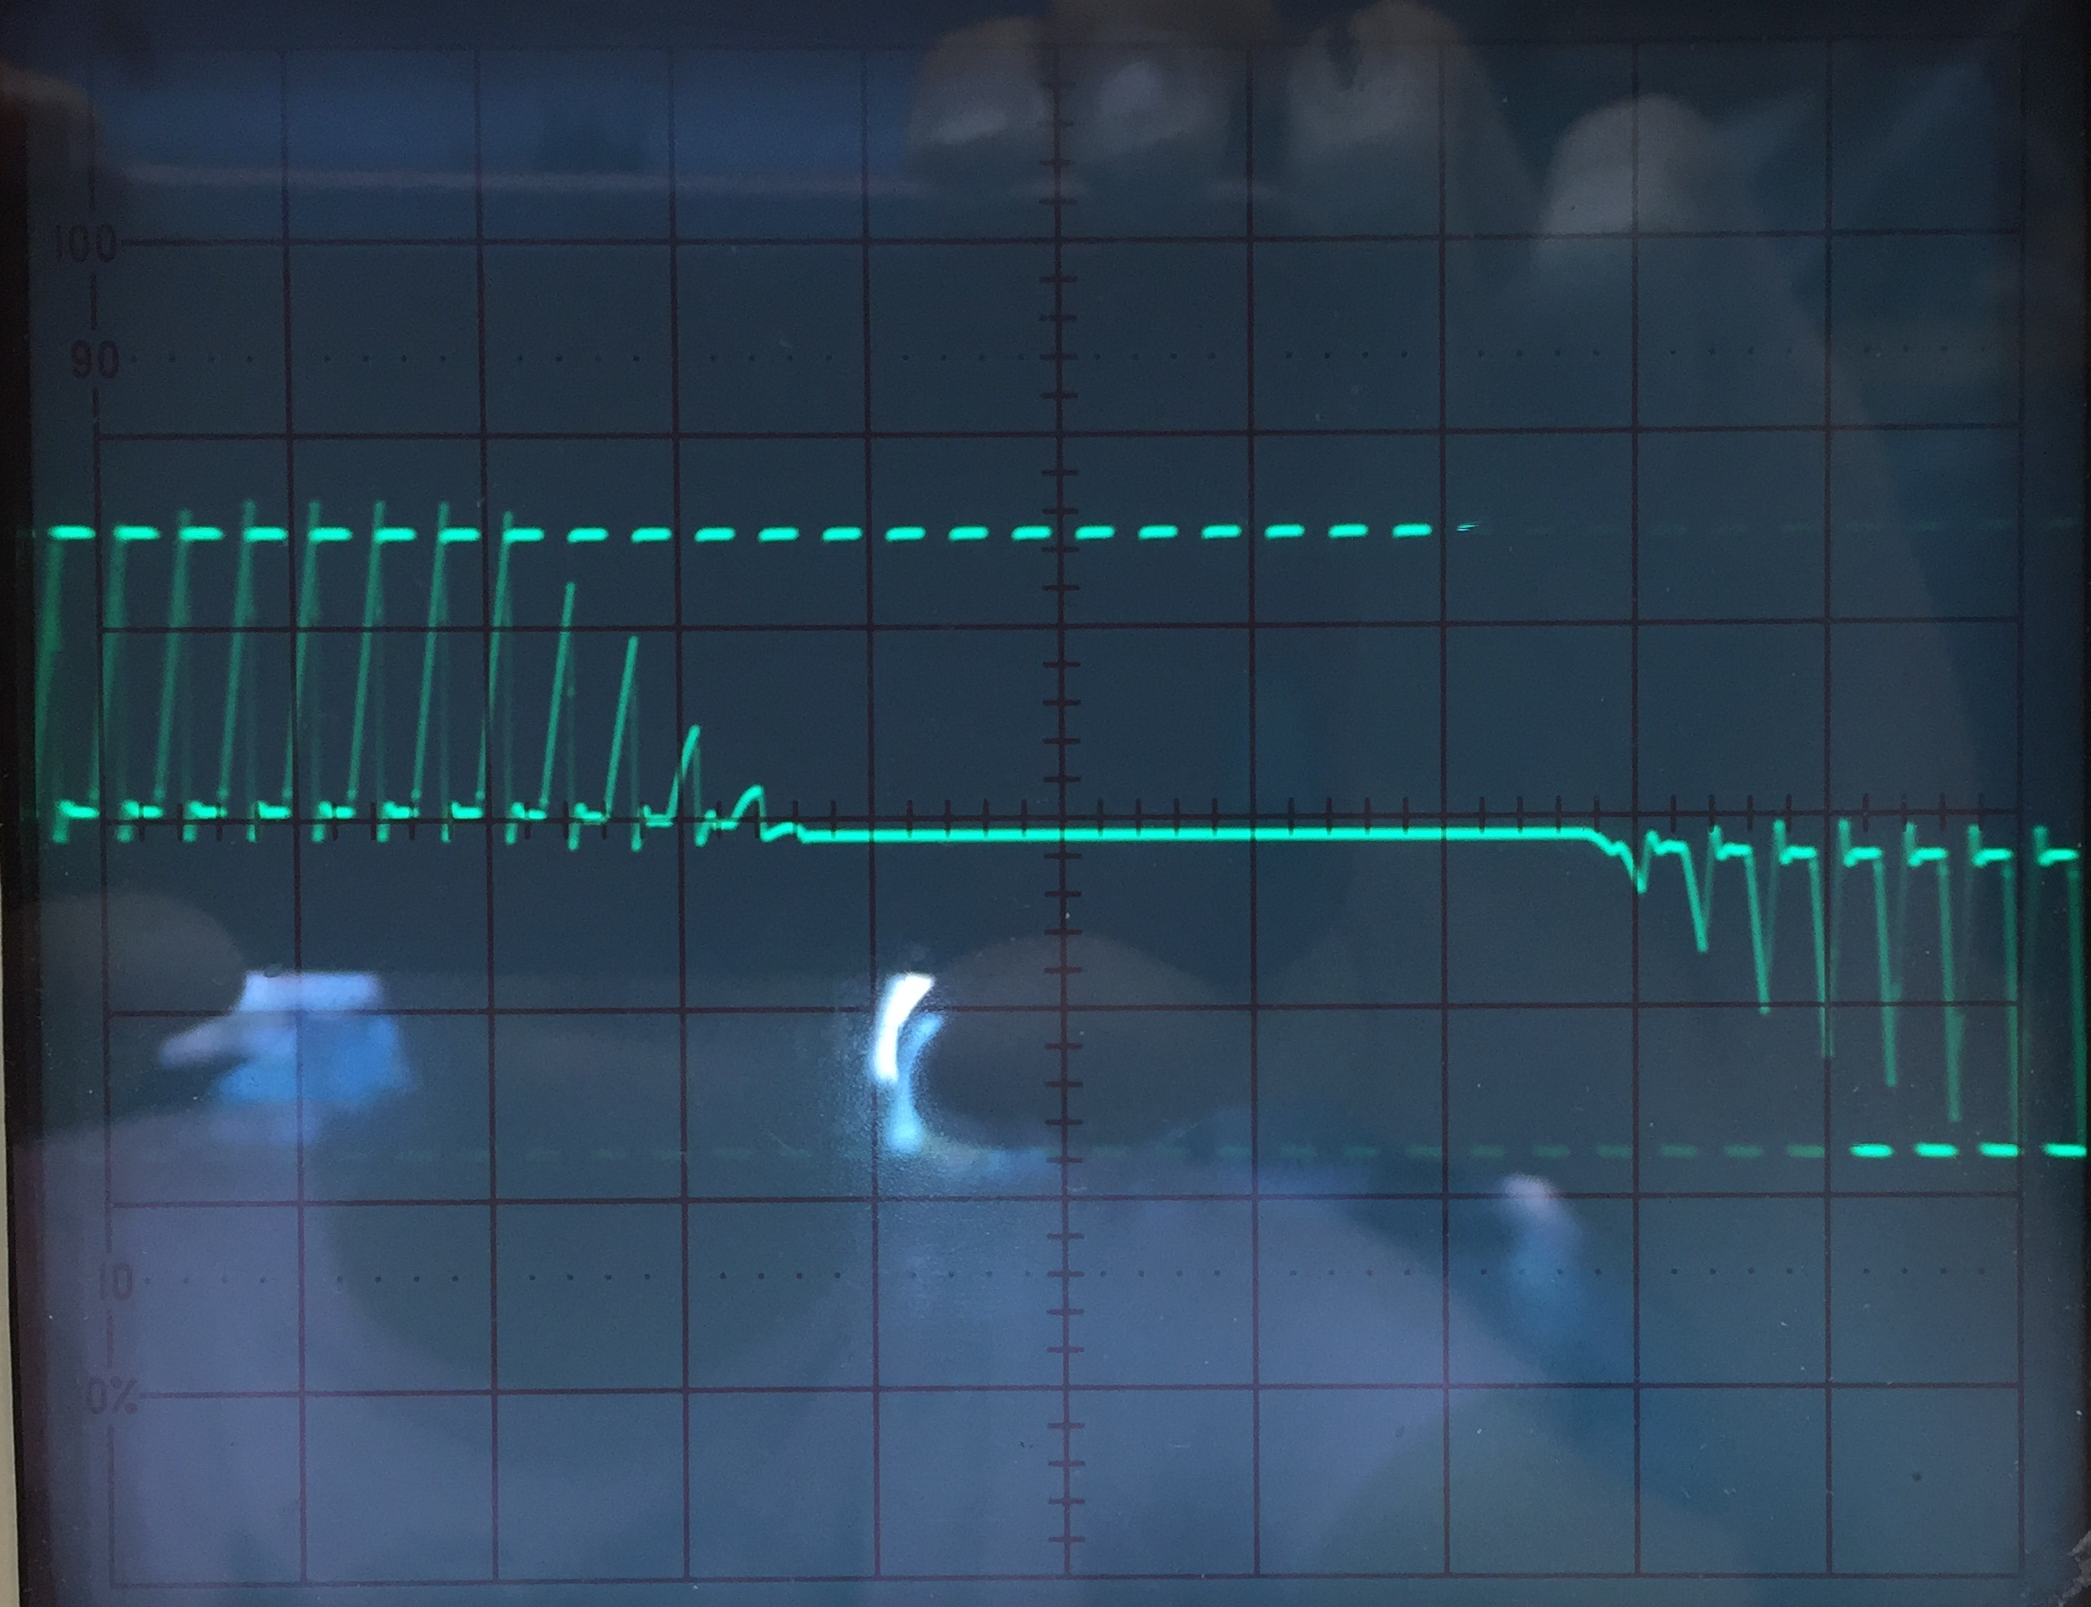
\includegraphics[width=60mm]
		{chapters/hardware-chapters/commercial-230v-ac-led-modulating-cropped.png}
	}

	\caption{Voltage measured over a 22 ohm series resistor at the primary side, to determine the current flow of a commercial 230 V AC LED.}
\end{figure}





Given the shortcomings of the existing hardware, it was decided to build custom hardware that would behave exactly how it was needed in order to successfully encode information in such a way that the currents could be decoded by a smart-meter.
In the following subsections each part of the hardware of the custom LED modulator will be explained.
The entire modulator's schematic can be found in \todo{Appendixxx}



	\subsubsection{Triggering}

	LEDs require a certain voltage to be present before they start to draw current.
	Since the provided AC is continuously changing its voltage, it must be known when that voltage is high enough in order for the LEDs to start drawing current.
	When the LEDs are not provided with enough voltage, there is no current draw and without the current draw, there can be no information encoding.
	The circuit that signals a microprocessor when the voltage is high enough can be found in \autoref{fig:custom-modulator-trigger}.
	The optocoupler makes sure that the AC is electrically isolated from the microprocessor.
	The output pin will be high voltage output, the provided voltage, when the AC voltage is higher than the preset and will be 0 V output when the AC voltage is below that preset.
	The preset can be determined by the potentiometer.

	%\begin{figure}[htb]
	%	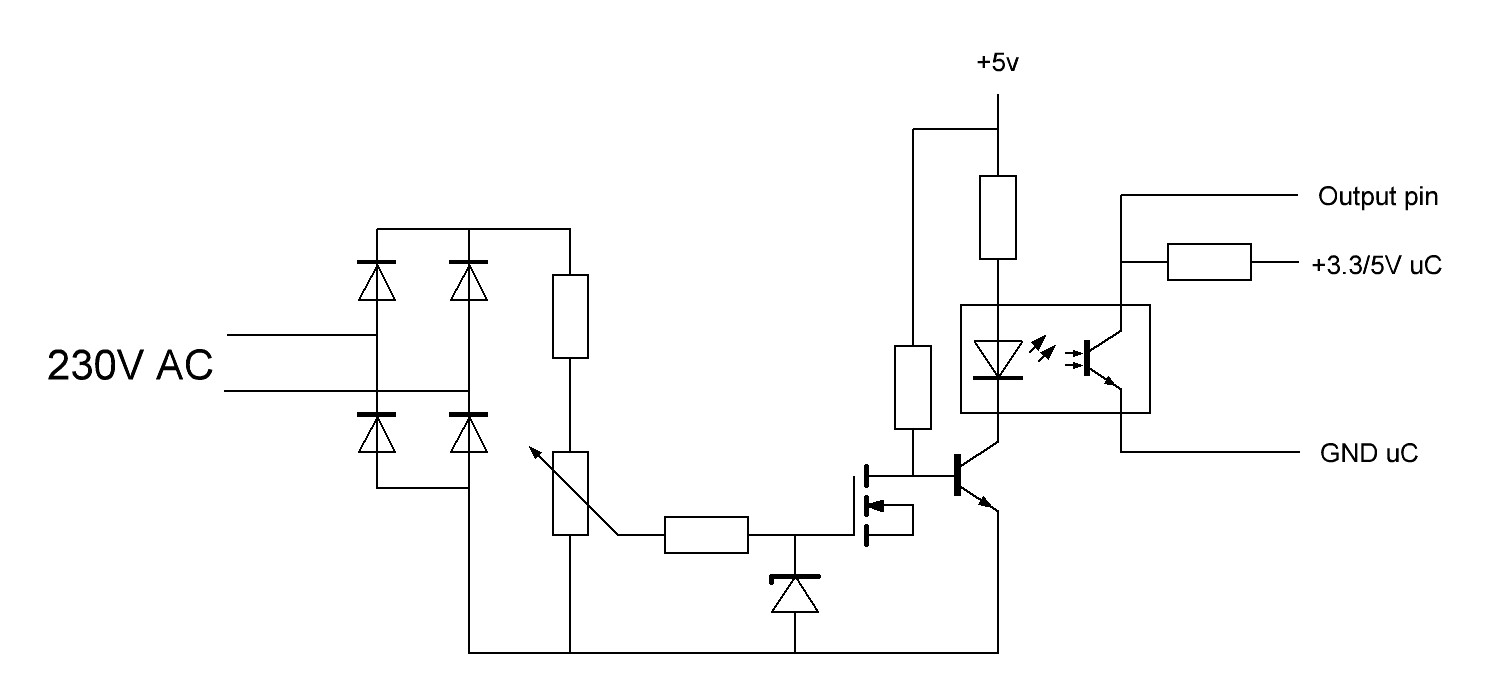
\includegraphics[angle=0,width=\textwidth]{chapters/hardware-chapters/custom-modulator-trigger.JPG}
	%	\caption{Triggering circuit to determine when the voltage is sufficiently high enough to start encoding information.}
	%	\label{fig:custom-modulator-trigger}
	%\end{figure}
	


	%Both figure side by side to save space...
	\begin{figure}[!tbp]
	  \centering
	  \begin{minipage}[b]{0.48\textwidth}
	    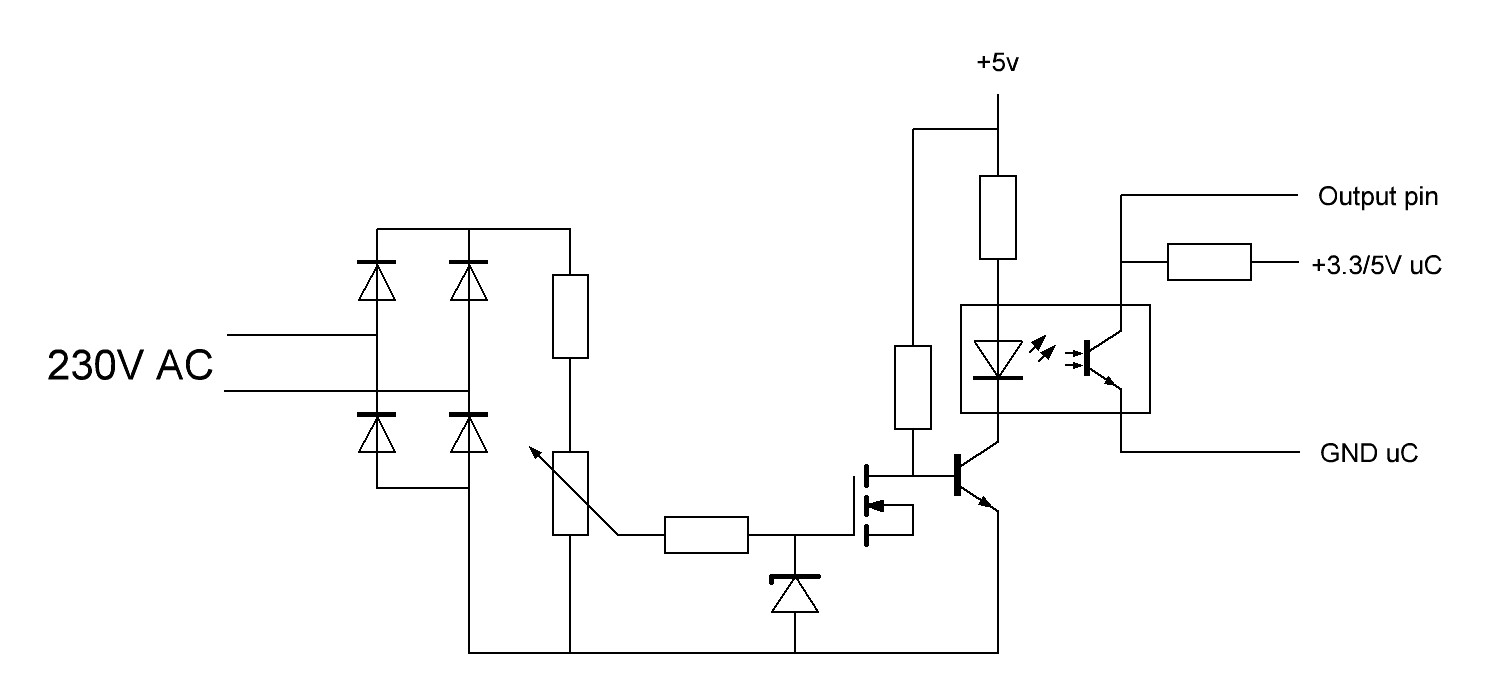
\includegraphics[width=\textwidth]{chapters/hardware-chapters/custom-modulator-trigger.JPG}
	    \caption{Triggering circuit to determine when the voltage is sufficiently high enough to start encoding information.}
		\label{fig:custom-modulator-trigger}
	  \end{minipage}
	  \hfill
	  \begin{minipage}[b]{0.48\textwidth}
	    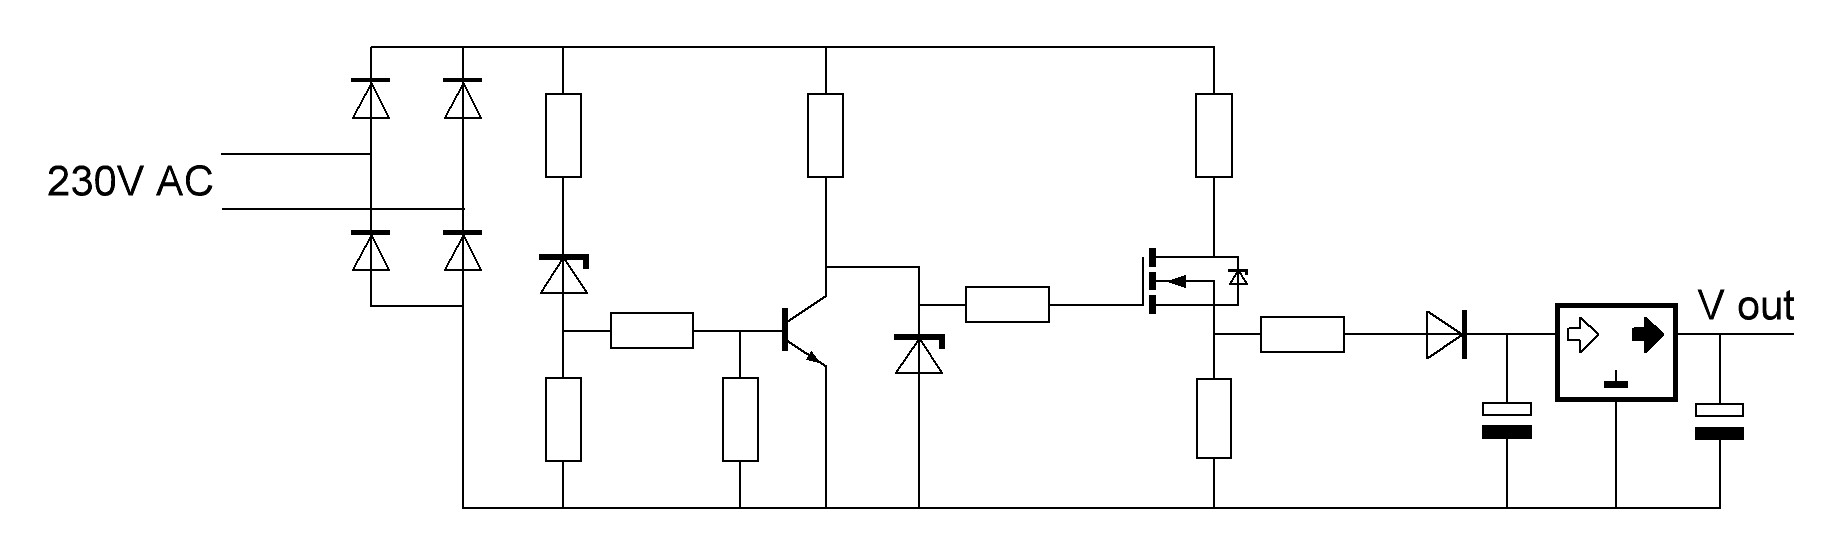
\includegraphics[width=\textwidth]{chapters/hardware-chapters/custom-modulator-voltage-source.JPG}
	    \caption{Non-disturbing voltage source to power other parts of the circuit.}
		\label{fig:custom-modulator-voltage-source}
	  \end{minipage}
	\end{figure}


	\subsubsection{Non-disturbing Voltage Source}
	\label{subsubsec:non-disturbing-voltage-source}

	The triggering circuit (\autoref{fig:custom-modulator-trigger}) requires a 5 V power supply.
	This voltage must be provided by a voltage source that will not distort the current draw.
	Otherwise it might disturb how the code sequence is translated in the current draw.

	Since the triggering circuit determines when the encoding may start, the voltage source can operate before the encoding starts.
	In that way it will not distort the encoding, because no encoding takes place yet.
	The schematic found in \autoref{fig:custom-modulator-voltage-source} provides a stable 5 V output.
	By only drawing current when there is no encoding being done, the voltage that the AC is providing is low, but still above 5 V.
	The AC voltage is then being used to charge a capacitor, that goes to a voltage stabilizer.
	The capacitor can then provide enough power for the triggering circuit until the capacitor can be charged again.


	%\begin{figure}[htb]
	%	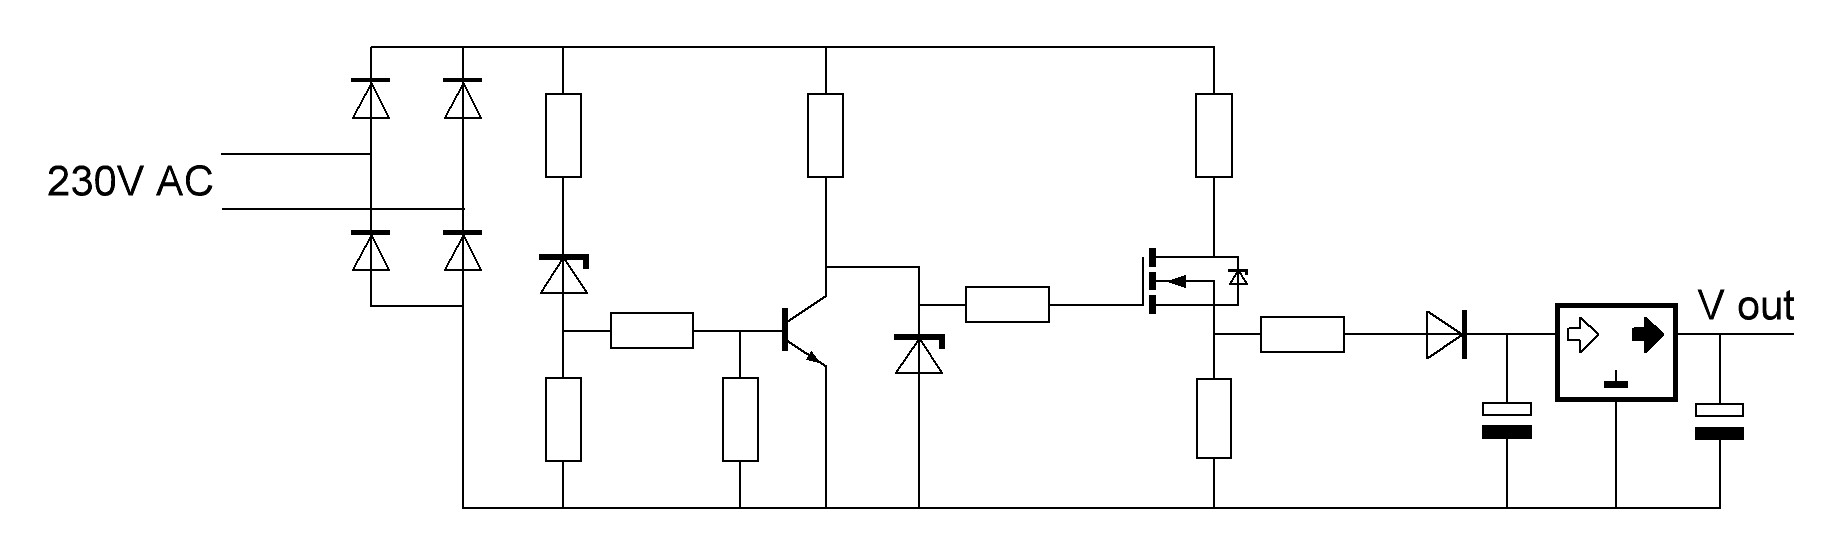
\includegraphics[angle=0,width=\textwidth]{chapters/hardware-chapters/custom-modulator-voltage-source.JPG}
	%	\caption{Non-disturbing voltage source to power other parts of the circuit.}
	%	\label{fig:custom-modulator-voltage-source}
	%\end{figure}



	\subsubsection{Current Source}


	For the current to be drawn instantaneously when the microprocessor tells the LED to turn on and to always be the same amount of current, a current source is implemented. 
	This will deal with the problems that the other hardware had, as can be seen in Figure \ref{fig:custom-modulator-voltage-source}.
	The toggling of the current source on and off must be isolated from the microprocessor, to protect the microprocessor in the development stages.
	The schematic can be found in \autoref{fig:custom-modulator-current-source}.
	\todo{Maybe add scope measurement of the actual current ....}


	\begin{figure}[htb]
		\centering
		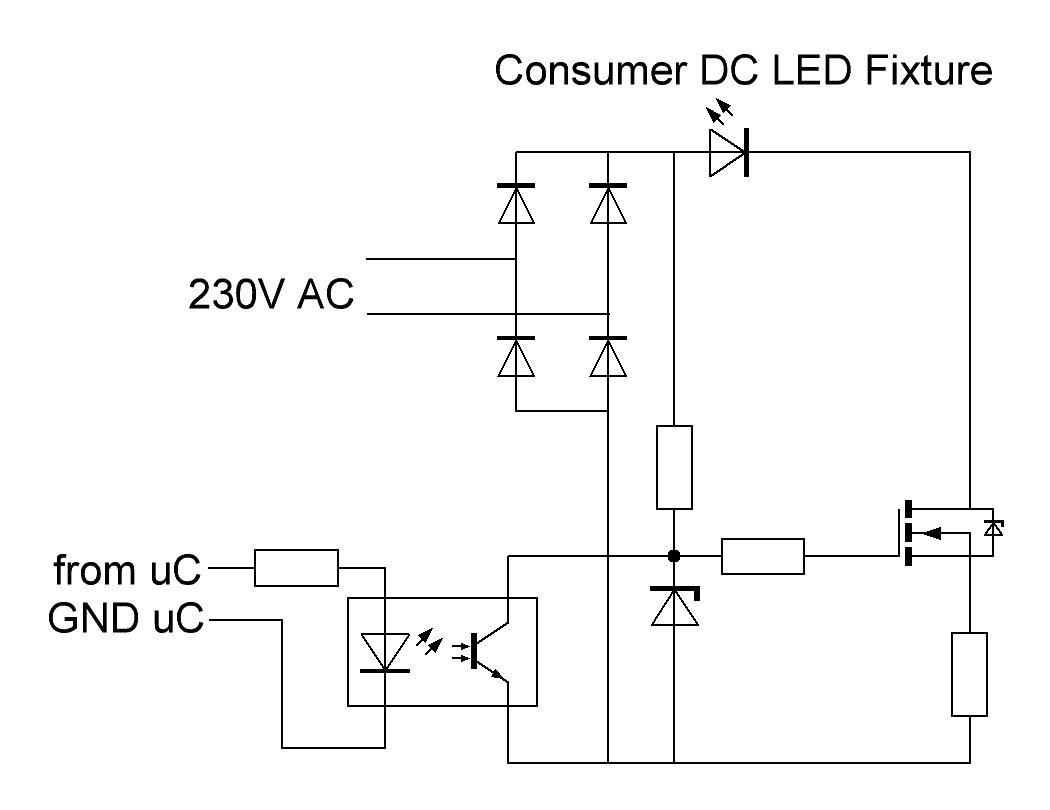
\includegraphics[angle=0,width=0.5\textwidth,keepaspectratio]{chapters/hardware-chapters/custom-modulator-current-source.JPG}
		\caption{Current source to power the commercial LED fixture, can be toggled on and off with a microprocessor.}
		\label{fig:custom-modulator-current-source}
	\end{figure}


\subsection{Current Sampler}

To measure AC current there are products on the market.
One such a product is a `Hall Effect-Based Linear Current Sensor'.
Based on the Hall effect, this sensor outputs a voltage which is linear dependent on the current that goes through the sensor.
The 230 V AC is magnetically decoupled from the output voltage, due to the Hall effect.
Since the AC current can be both positive and negative, the output voltage of the sensor is half of the applied $V_{cc}$ when no current is being drawn.
When the current is positive the output voltage can go up to the $V_{cc}$ and when the current is negative the output voltage can go down to the GND voltage. 
The output voltage can therefor be directly attached to the input of an ADC.


Unfortunately, this sensor has the issue that the noise is produces is too great for the sensitivity it has.
According to \cite{hall-ac-current-sensor-datasheet}, the highest sensitivity is $185$ mV / A.
The commercial LED fixtures which were provided, are rated at $15$ Watts.
With the 230 V AC, this works out to a current of $I = \frac{P}{U} = \frac{15}{230} = 0.065$ A.
At that current the output voltage will be $185 \times 0.065 = 12$ mV.
The noise of the output is $21$ mV, which is almost double the output voltage when one LED is on.
This sensor would not be able to reliably detect one or two LEDs.
And so it was decided that a series resistor would be used.

Because of the AC the voltage over the series resistor will be both positive and negative.
So the output voltage needs to be lifted up before it can go to an ADC.
When the voltage is within bound for the ADC, nothing is yet decoupled from the microprocessor.
So an isolation IC is used to isolate the external ADC from the microprocessor.

The current sampler also needs to know when to start looking for the encoded information.
Just like the LED modulator needs to know when to start encoding.
So the same triggering circuit is also used for the current sampler.

The full schematic of the current sampler can be found in \autoref{app:custom-current-sampler-schematic}.





\subsection{Testbed}
\label{subsec:ac-testbed}

The full AC testbed consists of three custom LED modulators with three (provided) commercial DC LED fixtures.
The modulators are connected in parallel. 
And in series is the custom current sampler to measure the current and decode the information that the modulators encode.
All micro-controllers are stand-alone.
In \autoref{fig:ac-test-bed-architectural}, the architectural overview can be seen of this testbed.

\begin{figure}[htb]
	\centering
	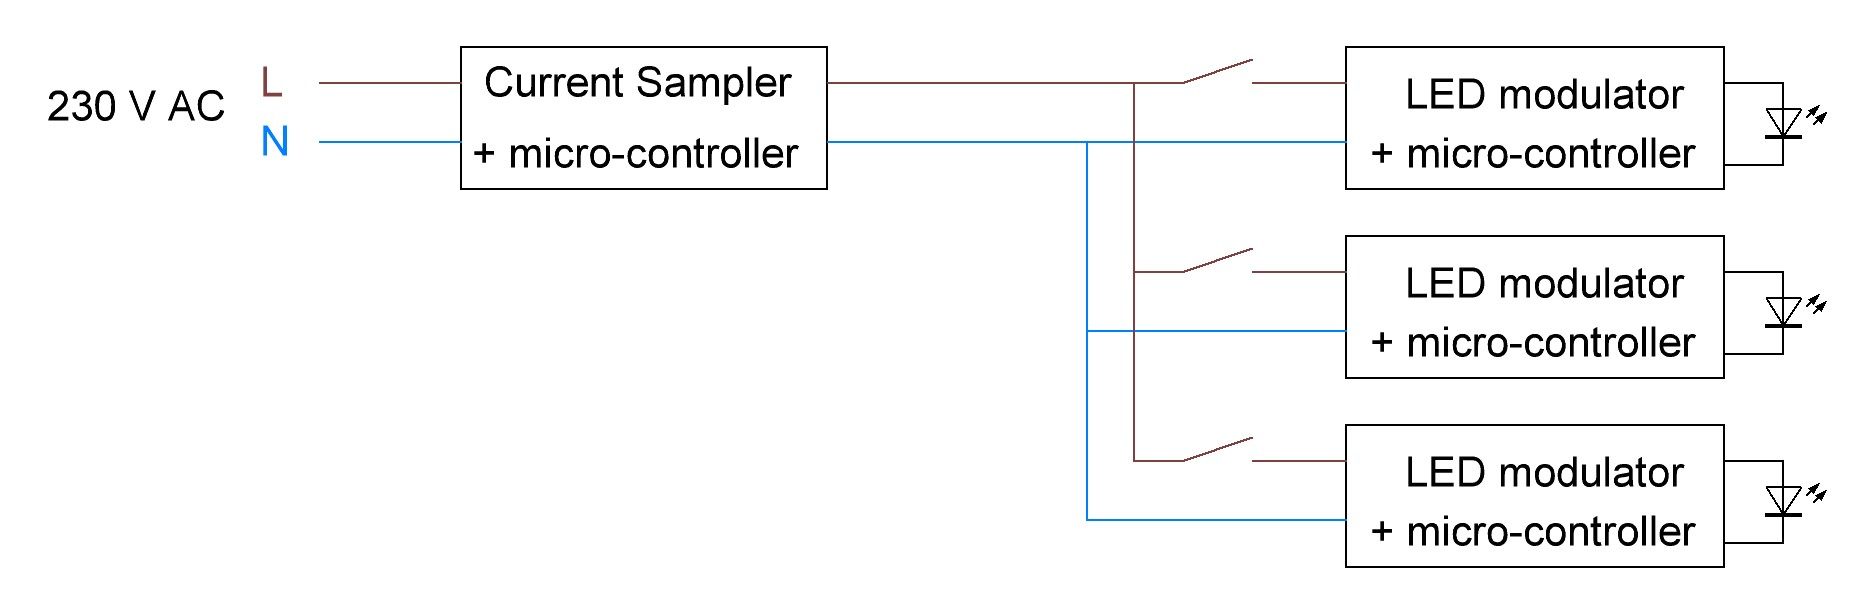
\includegraphics[angle=0,width=\textwidth,keepaspectratio]{chapters/hardware-chapters/ac-test-bed-architectural.JPG}
	\caption{Architectural overview of the AC testbed. Three LED modulators, with switches to turn the LED on and off, are connected in parallel with each other and in series with the current sampler.}
	\label{fig:ac-test-bed-architectural}
\end{figure}



